

When performing software tasks in large and complex software systems, software developers typically consult several different kinds of artifacts that assist them in their work~\cite{Starke2009, Meyer2017}. For example, 
when incorporating a new API library needed for a new feature, a developer might consult official API documents and guidelines~\cite{robillard2011field, umarji2008archetypal} or 
 question-and-answer forums for functionality, security and performance-related topics~\cite{parnin2012, silva2019}.



Much critical information in this and other non-source code types of artifacts 
contain data in the form of unstructured text~\cite{Bavota2016} and 
a developer must read the text to find the information that is \textit{relevant} to the task being performed.
However, the sheer amount of information \textit{within} these natural language artifacts may prevent a developer from comprehensively assessing what is useful to their task~\cite{Murphy2005}. Just within one kind of document, API
documentation, studies have shown that it can take 15 minutes or more
of a developer's highly constrained time to identify 
information needed to perform a particular software task~\cite{endrikat2014, Meyer2017}
and a developer that fails to locate all, or most, of the information needed
 will have an incomplete or incorrect basis from which to perform a software task~\cite{Murphy2005}.





\section{Scenario}
\label{cp1:example}




To illustrate challenges in locating information useful for a task, let us consider an open-source mail client\footnote{\url{https://github.com/k9mail/k-9}}.
Figure~\ref{fig:android-notifications-task} shows a task---in the form of a GitHub issue---that indicates that the app notifications 
are not working as expected\footnote{\url{https://github.com/k9mail/k-9/issues/1741}}. 


\begin{figure}[h!]
    \centering
    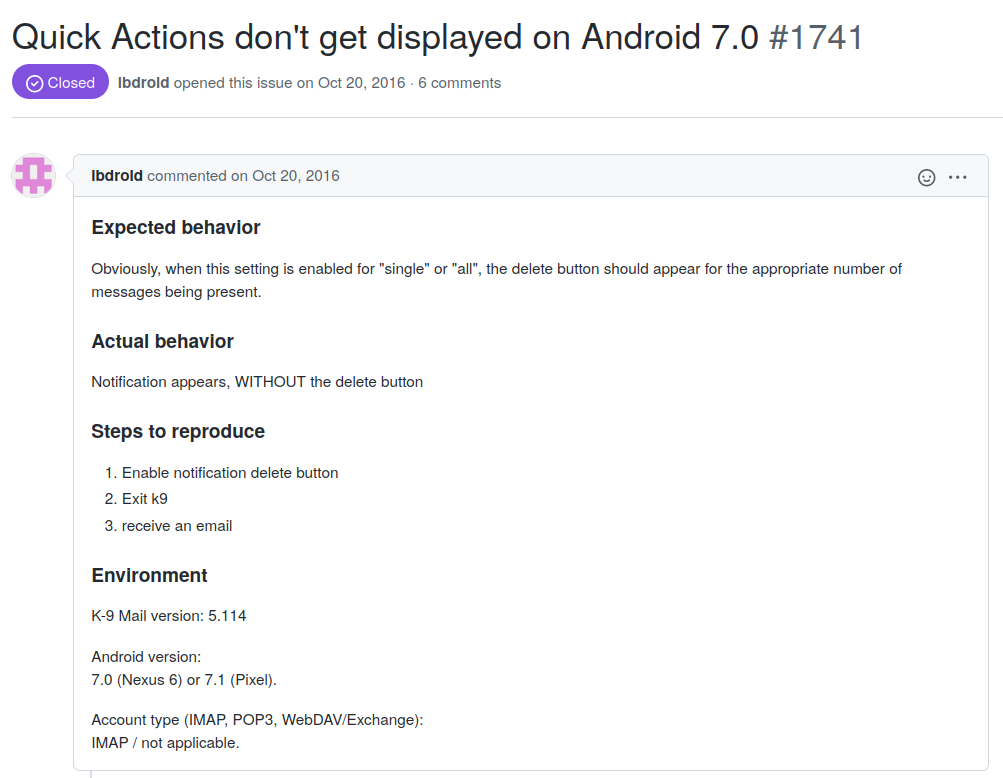
\includegraphics[width=.85\textwidth]{cp1/android-quick-actions}
    \caption{k-9 mail GitHub issue \#1741 indicating that quick actions don't get displayed on Android 7.0}
    \label{fig:android-notifications-task}
\end{figure}


A developer assigned to this issue might not be familiar with how Android notifications work and thus, they will need additional knowledge to understand and resolve the bug~\cite{ko2007, Li2013, sillito2006}. 
More than often, this knowledge can be acquired from a developer's peers~\cite{singer2011}. 
However, the fragmented and distributed nature of software development  
may prevent the developer from accessing their peers~\cite{ko2007},
what often makes  them seek online web resources for information 
that may assist them in completing the task-at-hand~\cite{Xia2017, rao2020}.
For example, the developer might use a web search engine to find software artifacts
pertinent to their task, such as the ones shown in 
Figure~\ref{fig:android-search-results}, which include a web tutorial, 
an API document, and a community forum web-page, respectively. 




\begin{figure}
    \centering
    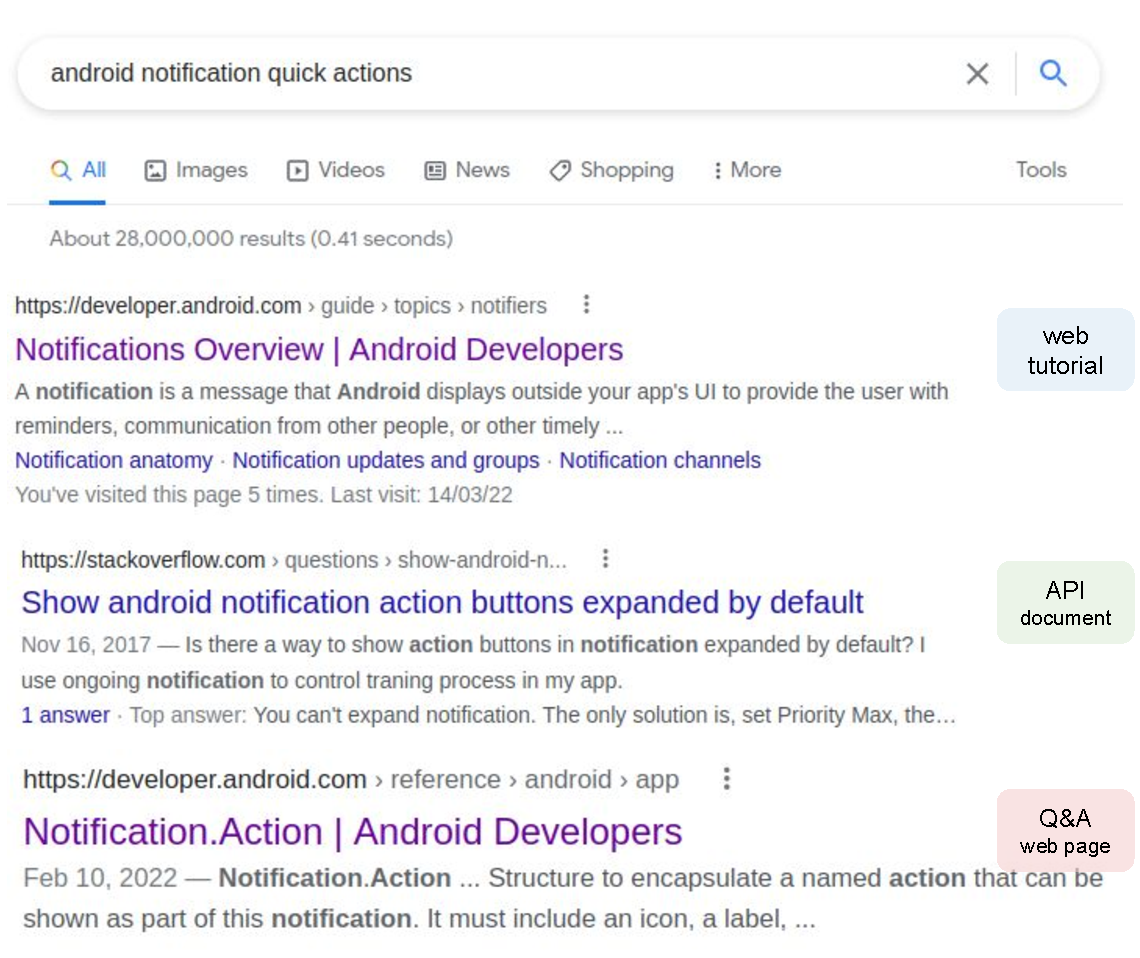
\includegraphics[width=.75\textwidth]{cp1/search-results.pdf}
    \caption{Search results showing artifacts of potential interest to the Android quick actions issue}
    \label{fig:android-search-results}
\end{figure}




Finding information useful to the developer's task 
 in these and other 
pertinent artifacts can be a time-consuming
and cognitively frustrating process~\cite{Begel2008,
robillard2011field}. 
Reading all of artifacts' content would take approximately 30 minutes or more\footnote{using a standard reading metric of 200 words per minute~\cite{Just1980}} of a developer's constrained time~\cite{endrikat2014, Meyer2017}
and not all of the content of these artifacts is relevant to the developer's task. 
For example, 
Figure~\ref{fig:android-create-notification} shows
that the Android notifications tutorial 
has information about both the Android versions 7.0 and 12.0 and, given the developer's task 
is related to the former version, only certain parts of this artifact  
(e.g., the text highlighted)
might be of relevance.





As tasks become more complex~\cite{Pirolli2007, Bystrom1995}, a developer also has to combine multiple pieces of text (from the same artifact or different ones) to understand what is needed for the task-at-hand~\cite{Piorkowski2016}. For example, Figure~\ref{fig:anatomy-of-relevant-text} gives further insight into 
how task-relevant text (i.e., the text highlighted)
is scattered across the web tutorial and the \acf{qa}
web page that the developer found in their search (Figure~\ref{fig:android-search-results})
for artifacts with information that could assist them in completing their task.
As we have described earlier in this chapter, if no tool support is provided, much of the process of finding this relevant text falls on the developer's shoulders~\cite{gonccalves2011, Ko2006a, Bystrom1995}.



Researchers have long recognized the value of 
 assisting developers in locating information in the natural language artifacts sought as part of a software task,
proposing many tools and approaches 
that combine \acf{IR}, \acf{NLP} and \acf{ML} techniques to identify potentially useful text in certain kinds of artifacts. 
For example, Nadi and Treude consider 
that relevant information in \acs{qa} 
web pages is often found in text with
conditional clauses (i.e., sentences with the word `\textit{if}')~\cite{nadi2020}
while Robillard and Chhetri assume that relevant 
text in API documents mention a code elements (e.g., a class name or method signature)~\cite{Robillard2015}, using such assumptions and a set of regular expressions 
for automatically identifying relevant text.
As another example, both Xu et al.~\cite{Xu2017} 
and Silva et al.~\cite{silva2019} use 
structured data available on each of the answers in a Stack Overflow post 
(i.e., number of votes or whether an answer is the accepted answer)
as part of their approaches to identify relevant text.



Although effective in specific contexts,
the assumptions in these and other techniques mean that:

\begin{itemize}
    \item they may fail to locate part of the relevant text; for example, the relevant text in the \acs{qa} web page shown in Figure~\ref{fig:anatomy-of-relevant-text} does not contain conditional clauses; likewise, not all of the relevant text in the API tutorial contains code elements;
    \item they might not apply across the
    many different kinds of artifacts a developer may encounter
    daily in their work~\cite{Li2013}, i.e., all to often, the structure of 
    the artifacts sought by a developer differ, thus requiring specialized 
    approaches for each type of artifact.
\end{itemize}


This scenario illustrates thus some of the challenges in locating task-relevant textual
information and motivating the need for more generalizable techniques.



\clearpage


% https://tex.stackexchange.com/questions/468393/including-large-images-in-landscape-formatting
\begin{landscape}
\begin{figure}
    \centering
    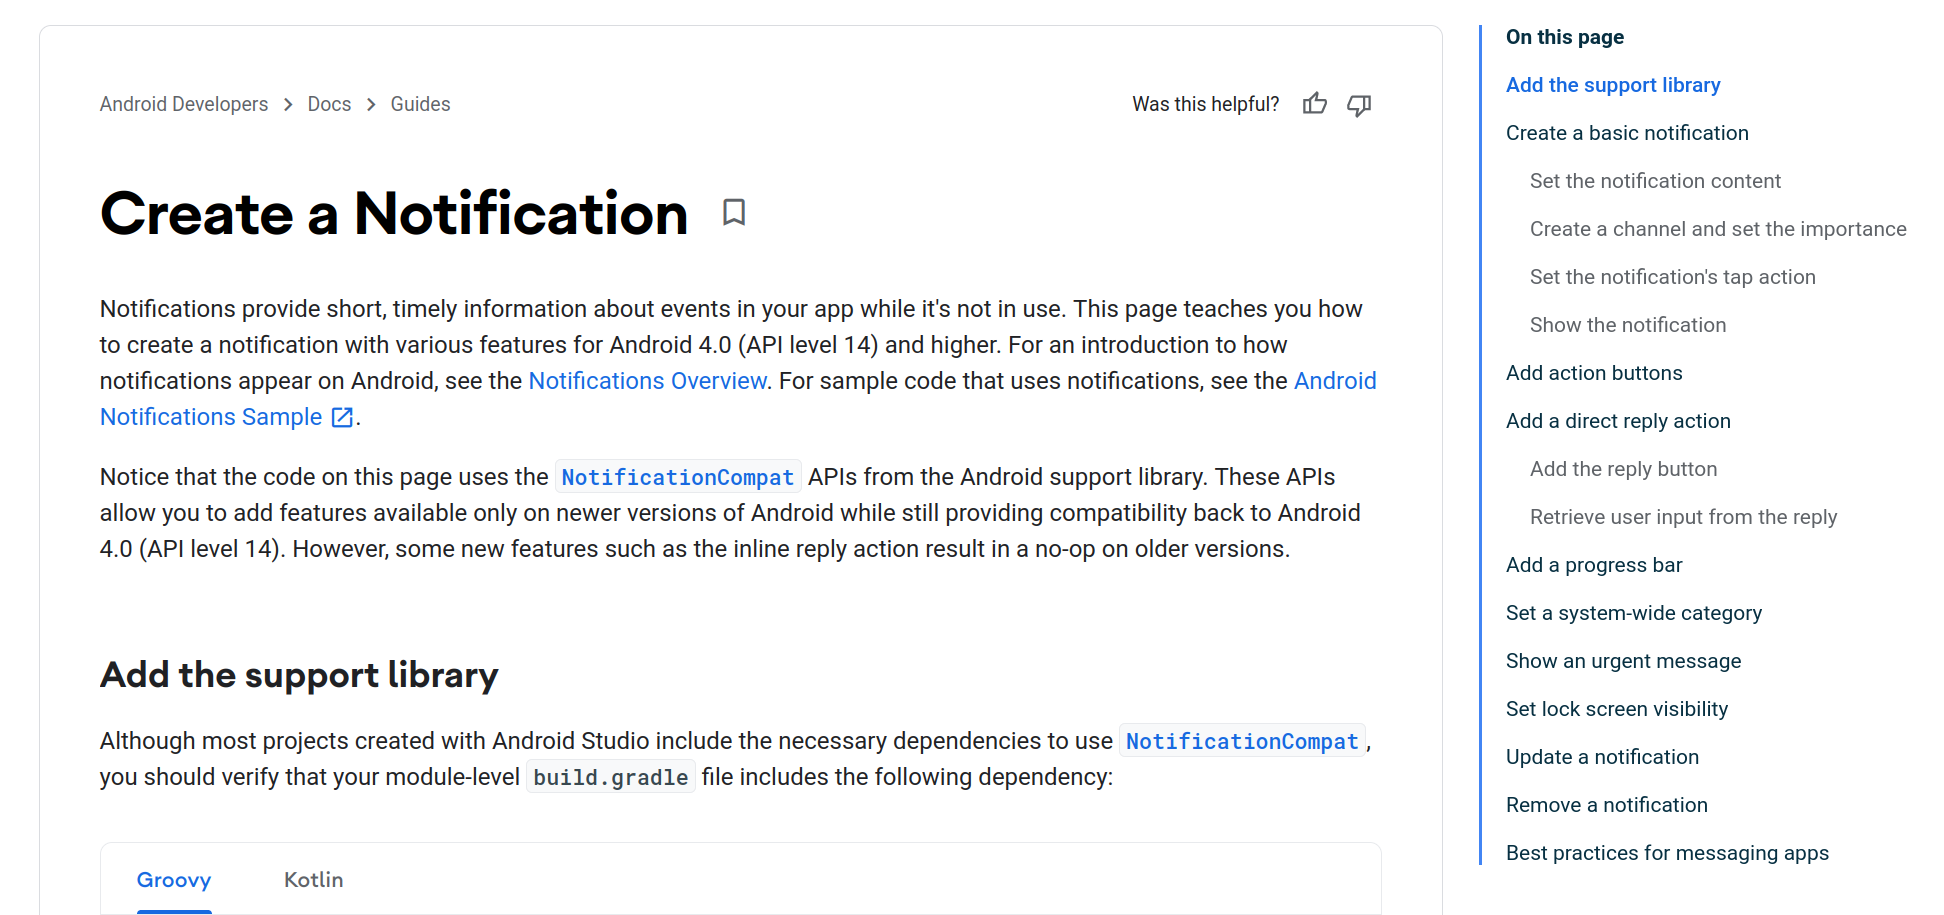
\includegraphics[width=\dimexpr\linewidth-4\fboxsep-2\fboxrule]{cp1/create-notification.png}
    \caption{Snapshot of the official Android notifications API overview}
    \label{fig:android-create-notification}
\end{figure}
\end{landscape}


\begin{landscape}
\begin{figure}
    \centering
    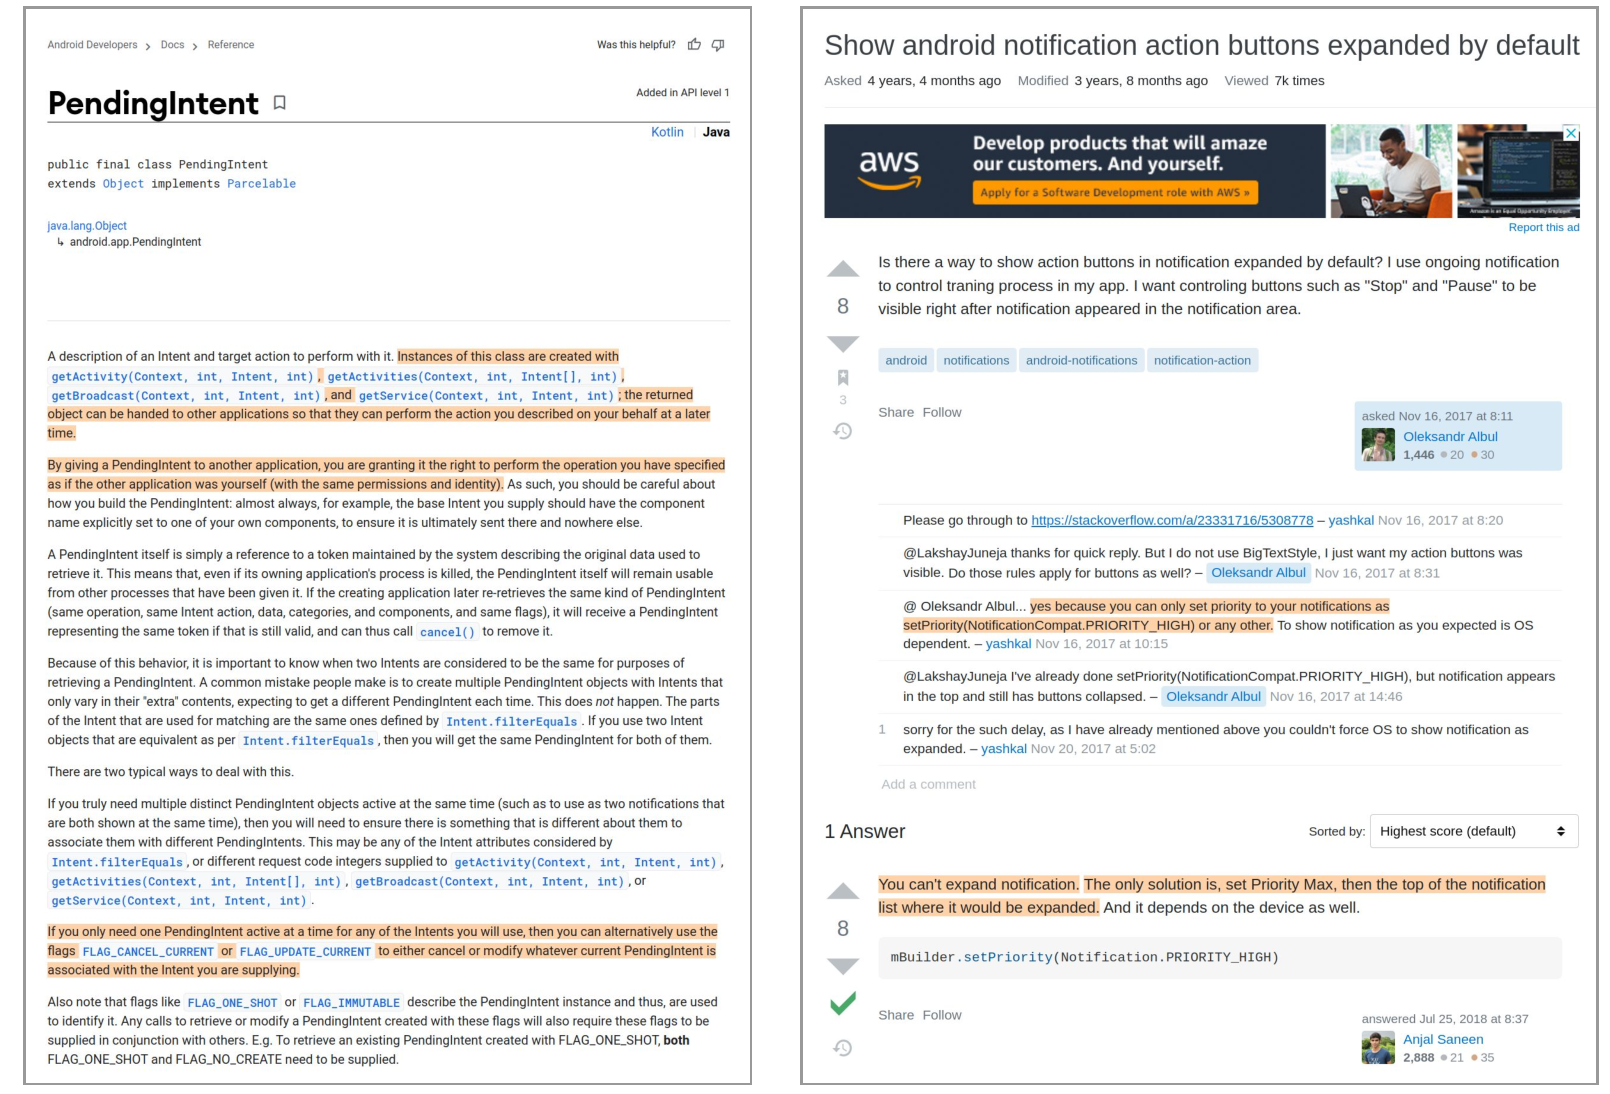
\includegraphics[width=\dimexpr\linewidth-4\fboxsep-2\fboxrule]{cp1/notifications-relevance.pdf}
    \caption{Relevant text for the Android notifications task found across different kinds of artifacts, i.e., a web tutorial (on the left) and a question-and-answer web page (on the right) }
    \label{fig:anatomy-of-relevant-text}
\end{figure}
\end{landscape}

\clearpage


% \clearpage


% a snapshot 
% of the Android notifications documentation, where among  
% the many topics presented on the page (right-hand side), only the `\textit{notification actions}' portion (under focus) might be rof relevance.
% This illustrates the burden of sifting through large amounts of
% irrelevant text (e.g., because of legacy information, boilerplate text, or because it is intended for another audience) to filter just those parts that are relevant to a developer~\cite{Robillard2015}. 











% about adding
% action to a notification is found across multiple artifacts.
% If no tool support is provided, much of the process of navigating through artifacts of interest and locating text 
% relevant to a task fall on the developer's shoulders~\cite{gonccalves2011, Ko2006a, Bystrom1995}.






% Researchers have long recognized the value of assisting developers in 
% identifying information of relevance within the natural language
% text of a software artifact






% but such a technique would fail to locate the relevant text 
% shown in Figure~\ref{fig:anatomy-of-relevant-text}.


% consider pre-defined kinds of tasks or types of artifacts.
% For example, {\small DeMIBuD}~\cite{Chaparro2017} is a technique that applies to bug reports and 
% assists in bug triaging. Although valuable, the text   detailing a bug's observed or expected
% behaviour and automatically identified by this tool
%  is of little help to a developer who accessed that bug 
% with the hope that the bug's solution also applies to their current task~\cite{Viviani2019}.





% 
\vspace{3mm}
\begin{figure}
\centering    
\parbox{\textwidth}{% 
\centering
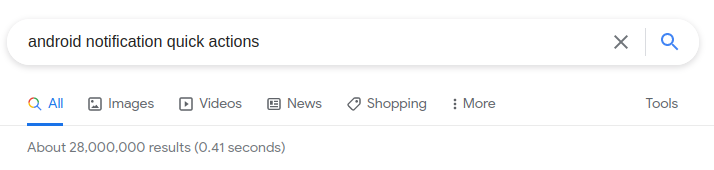
\includegraphics[width=.80\textwidth]{cp1/task-google-search}
}
\parbox{\textwidth}{%
\centering
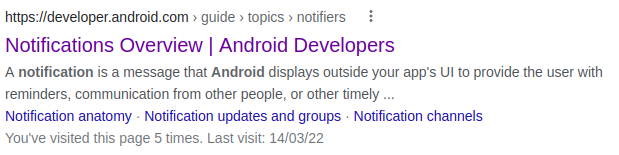
\includegraphics[width=.70\textwidth]{cp1/api-documentation-search-result}
}
\parbox{\textwidth}{%
\centering
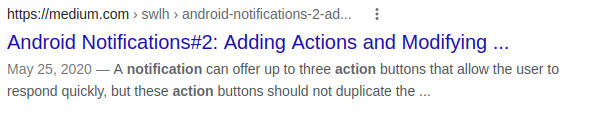
\includegraphics[width=.70\textwidth]{cp1/misc-documentation-search-result}
}
\parbox{\textwidth}{%
\centering
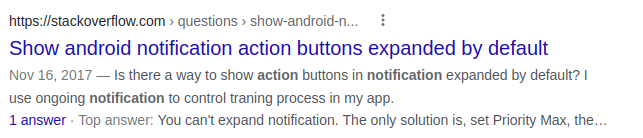
\includegraphics[width=.70\textwidth]{cp1/so-documentation-search-result}
}
\parbox{\textwidth}{%
\centering
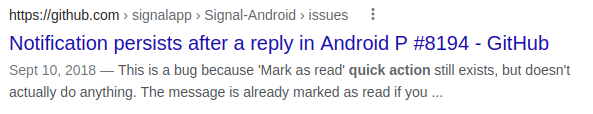
\includegraphics[width=.70\textwidth]{cp1/git-documentation-search-result}
}
\caption{Search results showing artifacts of potential interest to the Android quick notifications issue}
\label{fig:android-search-results}
\end{figure}







% While it is impractical to anticipate all the information needs a developer might have~\cite{sillito2006, josyula2018, ko2007}, there is an increasing interest in using the information 
% available in a software task for the purposes of automatically identifying text 
% which might assist in completing that task~\cite{Bavota2016}. 
% In such context, most of the approaches proposed by software engineering researchers 
%  only apply to certain kinds of artifacts, such as Stack Overflow posts~\cite{Xu2017, silva2019}, 
%  and use structural data available in these artifacts (e.g., extracting text only from top ranked answers)  to assist in the identification of relevant text
 
% These assumptions limit using such techniques across the
% many different kinds of artifacts a developer may encounter
% daily in their work~\cite{Li2013}, 
% illustrating thus some of the challenges in locating task-relevant textual
% information and motivating the need for more generalizable techniques.





% \begin{landscape}
% \begin{figure}
%   \centering
%   \begin{minipage}{.5\textwidth}
%       \centering
%       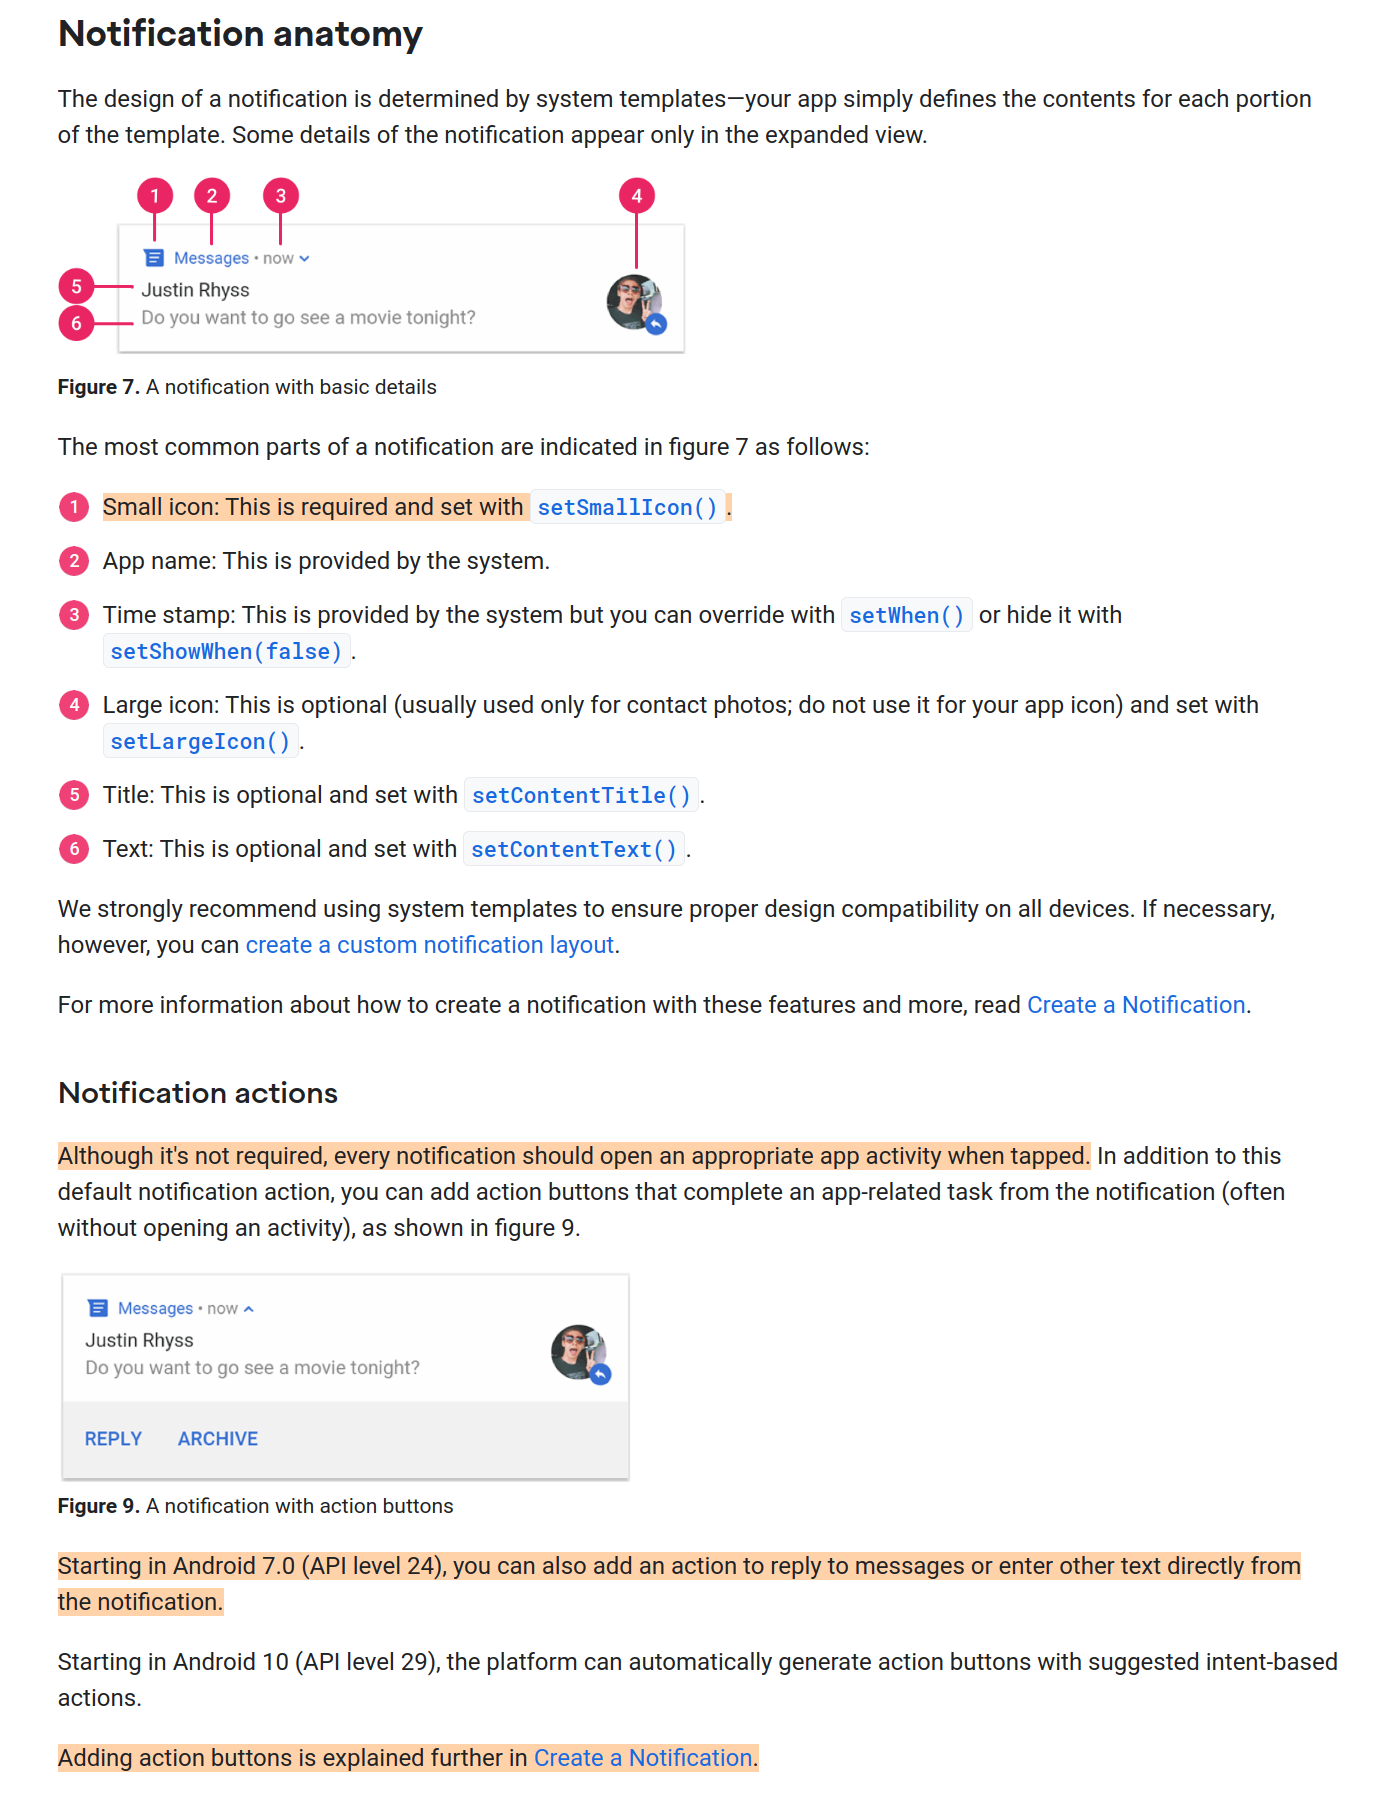
\includegraphics[width=0.5\linewidth, height=0.2\textheight]{cp1/notification-anatomy}
%     %   \caption{The Skip-gram model architecture~\cite{Mikolov2013}}
%     %   \label{fig:skip-gram}
%   \end{minipage}%
%   \begin{minipage}{0.5\textwidth}
%       \centering
%       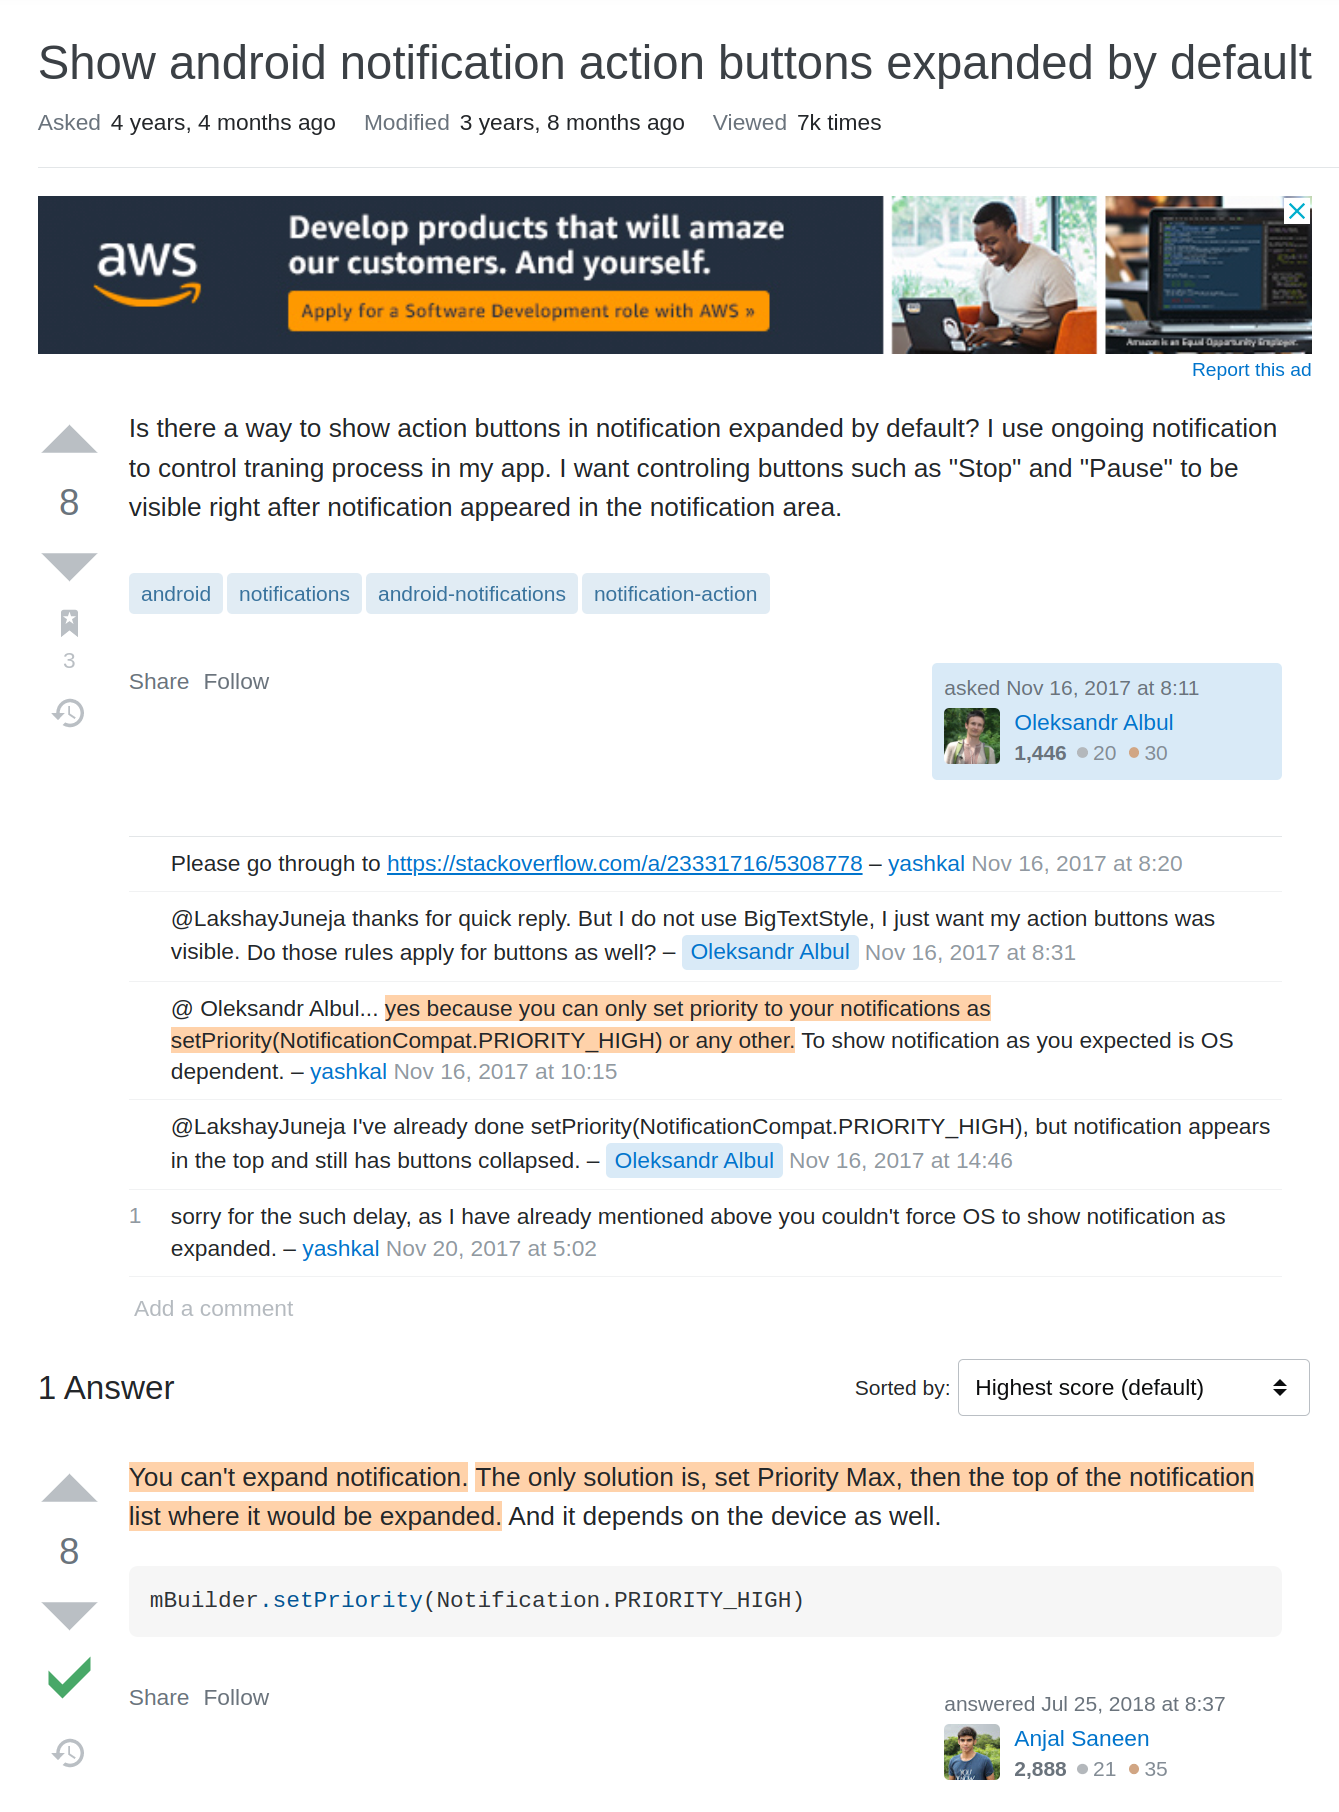
\includegraphics[width=\linewidth, height=0.2\textheight]{cp1/expand-notifications}
%     %   \caption{Positive and negative training examples~\cite{Ye2016}}
%     %   \label{fig:skip-gram-example}
%   \end{minipage}
% \end{figure}
% \end{landscape}





% Some \acs{NLP} techniques rely on regular expressions describing a sequence of tokens
% representing words or linguistic elements 
% often found in relevant text~\cite{Bavota2016, Chaparro2017}.
% Other \acs{ML}-based techniques use extractive text summarization 
% to produce a summary of an artifact's content~\cite{Lotufo2012, Ponzanelli2015}
% and a developer might use this summary to find key information
% that may help them complete their task~\cite{Bavota2016}.